\chapter{Iteración 4}
\section{Objetivos de iteración}
\begin{itemize}
  \item Integración de MongoDB (como contenedor docker) 
  \item Cliente más avanzado. Servidor estructurado en Servicio / Controlador.
\end{itemize}

\section{Integración de MongoDB}
\emph{MongoDB} es una base de datos no relacional (\emph{NoSQL}) basada en documentos y
que utiliza \emph{JSon} como formato de intercambio de información.

La integración se ha realizado mediante un contenedor \emph{Docker} de forma que tanto el
desarrollo como el despliegue es fácilmente reproducible.

El servidor GameRegistry necesita una instancia de \emph{MongoDB} para funcionar.
La integración, realizada mediante el módulo \emph{Vertx} llamado \emph{MongoDB persistor}, depende
de un archivo de configuración para obtener los datos relativos a la conexión con \emph{MongoDB}.
Cambiando los parámetros de este archivo de configuración es posible hacer que el servidor
GameRegistry se conecte a una u otra instancia de \emph{MongoDB}.

Hay que tener en cuenta que el contenedor de \emph{MongoDB} utiliza un \emph{Volumen} (un espacio
de almacenamiento ``externo'' al contenedor que persiste de un lanzamiento a otro). A menudo es
conveniente configurar el lanzamiento del contenedor de \emph{MongoDB} de forma que dicho volumen
corresponda a una carpeta del host:

\texttt{\$ docker run -v [local path]:/data/db/ --name mongo-server mongo:3.0.1}

donde \texttt{local path} es la ruta a una carpeta del host que será utilizada por \emph{Docker}
para montar la carpeta \texttt{/data/db} en el contenedor de \emph{Docker}. De este modo
los archivos relativos a la base de datos de \emph{MongoDB} quedan fuera del contenedor y es
posible examinarlos de forma externa o hacer copias de seguridad fácilmente.

\subsection{MongoDB y desarrollo}
Para desarrollar el servidor GameRegistry o lanzarlo de forma local fuera de un entorno
de contenedores \emph{Docker} tan solo es necesario obtener una instancia de \emph{MongoDB}
a la que se pueda conectar y un archivo de configuración con la información necesaria para
la conexión.

En el archivo \textbf{Readme.md} hay información básica sobre cómo conseguir una instancia
de MongoDB utilizando \emph{Docker}, que resulta a menudo más conveniente que instalar una
instancia local del mismo.

Hay que tener en cuenta que los contenedores de \emph{Docker} por defecto no exponen los puertos
al host. Las instrucciones básicas para lanzar \emph{MongoDB} como contenedor para desarrollo 
serían:

\begin{itemize}
 \item Descargar el contenedor (sólo la primera vez): \\
       \texttt{\$ docker pull mongo:3.0.1}
 \item Lanzar la instancia de \emph{MongoDB} exponiendo el puerto al host: \\
       \texttt{\$ docker run -P mongo:3.0.1}
 \item Modificar la configuración de GameRegistry si es necesario en el archivo \emph{conf.json}
 \item Lanzar el servidor GameRegistry: \\
       \texttt{\$ ./gradlew runMod -i}
\end{itemize}

\subsection{MongoDB y despliegue}
El \emph{Dockerfile} que describe cómo construir el contenedor de nuestro servidor GameRegistry
ha sido actualizado para integrar un archivo de configuración separado dedicado al contenedor 
llamado \emph{conf-docker.json}. Este archivo contiene la configuración necesaria (mínima) para
poder conectar con un servidor \emph{MongoDB} que corre en una máquina llamada \texttt{mongo-server}.
Esto resulta conveniente en un entorno \emph{Docker} enlazando ambos contenedores. Por ejemplo:

\begin{itemize}
 \item Descargar el contenedor de \emph{MongoDB} (sólo la primera vez): \\
       \texttt{\$ docker pull mongo:3.0.1}
 \item Lanzar la instancia de \emph{MongoDB} sin exponer puertos al host y nombrando la instancia del contenedor: \\
       \texttt{\$ docker run --name mongo-server mongo:3.0.1}
 \item Construir el contenedor para nuestro servidor: \\
       \texttt{\$ docker build -t distributedsystems/gameregistry .}
 \item Lanzar el contenedor de GameRegistry enlazándolo con el de la instancia de \emph{Docker} de forma
       que compartan la pila de red (y puedan así comunicarse), exponiendo el puerto de GameRegistry en el host: \\
       \texttt{\$ docker run -p 8080:8080  \\--link mongo-server:mongo-server distributedsystems/gameregistry}
\end{itemize}

\subsection{Distinción de dominio, controlador y servicio}
\begin{description}
  \item[Dominio] \hfill \\
  Clases POJO con el mismo esquema de la base de datos.
  \item[Controlador] \hfill \\
  Manejar los requisitos y respuestas y comunicar con el servicio.
  \item[Servicio] \hfill \\
  La lógica de negocio. Almacenar las sessiones en el base de datos.
\end{description}

\section{Diagrama de paquetes}
\begin{figure}[h]
 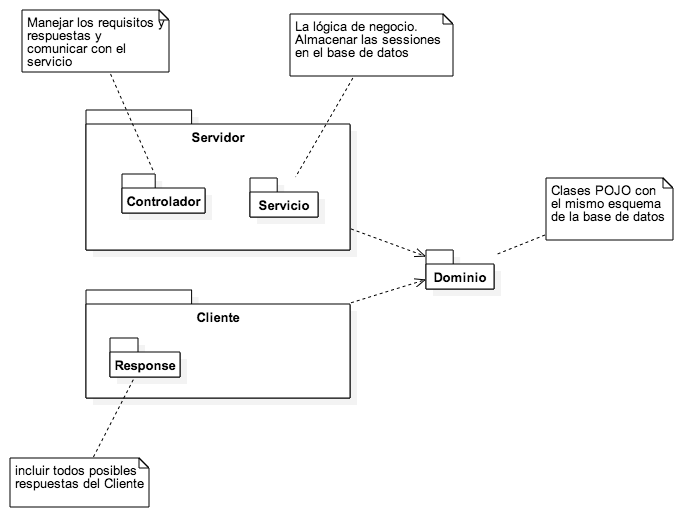
\includegraphics[scale=0.6]{diagrams/package_diagram.png}
 \caption{Organización de paquetes}
 \label{fig:paquetes}
\end{figure} 

\section{Diagrama de clases}
\begin{figure}[h]
 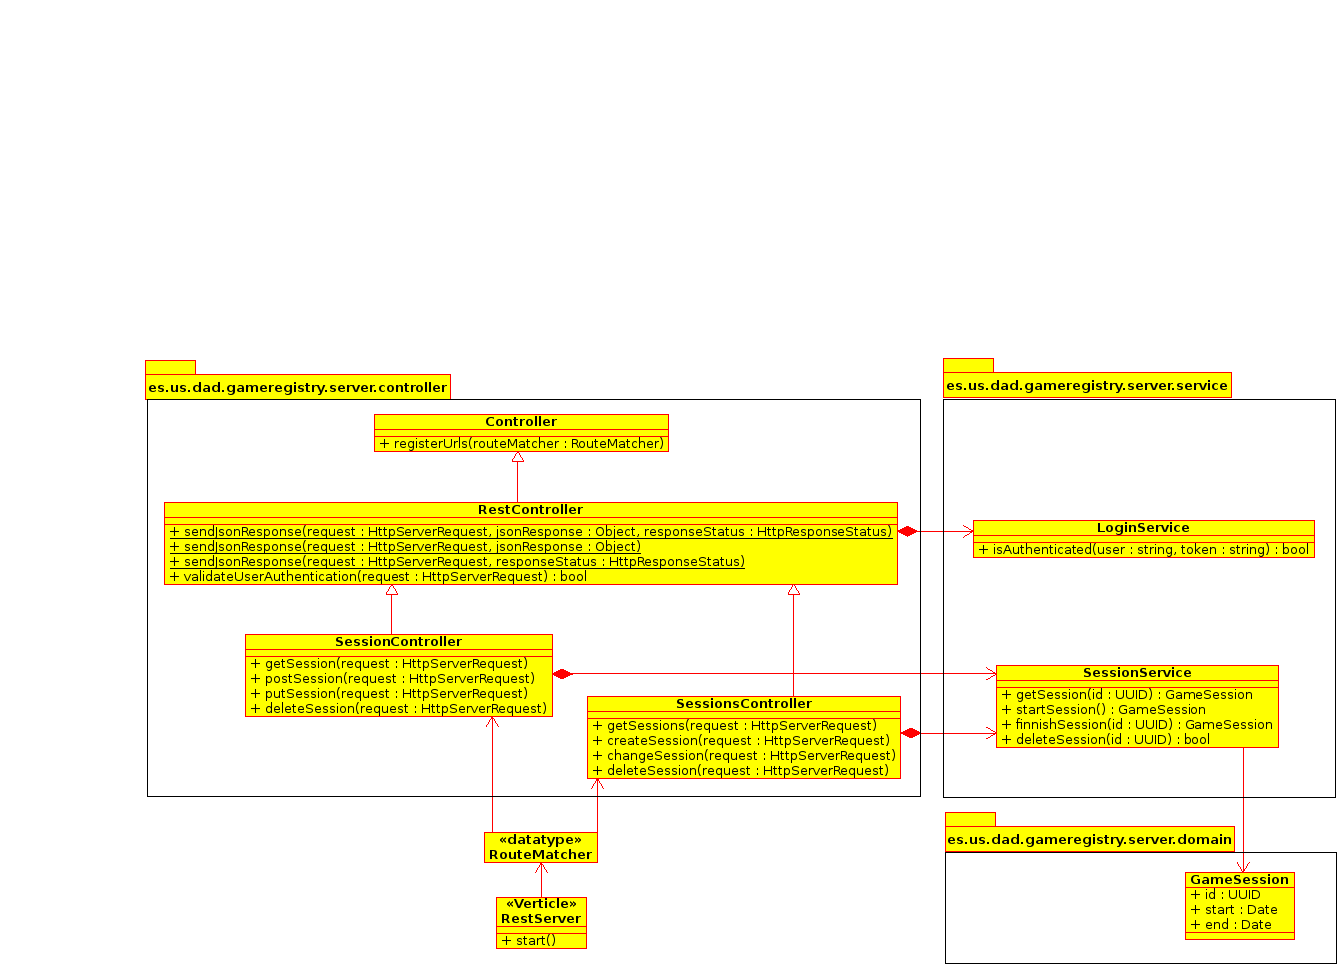
\includegraphics[scale=0.4]{diagrams/class_diagram_iter4.png}
 \caption{Diagrama de clases actualizado (iteración 4)}
 \label{fig:clases}
\end{figure}

